\documentclass[pdf]{beamer}
\mode<presentation>{} 

\usepackage{enumitem}
\usepackage{graphicx}
\usepackage{bbding}
\usepackage{pifont}
\usepackage{hyperref}
\usepackage{pgf}
\usepackage{tikz}
\usepackage{tikz-qtree,tikz-qtree-compat}
\usetikzlibrary{trees}
\usetikzlibrary{arrows,automata}
\usetikzlibrary{automata,positioning}
\usetikzlibrary{shapes}
\usepackage{pgfornament}
\usepackage{eso-pic}
\usepackage[absolute,overlay]{textpos}
\usepackage[scaled=1]{helvet}
\usepackage{times}
\usepackage{courier}
\usepackage{rotunda}
\usepackage{mathtools,enumerate,amssymb}
\usepackage[utf8]{inputenc}
\usepackage[T1]{fontenc}
\usepackage{color}
\usepackage{overpic}
\usepackage{minibox}
\usetikzlibrary{patterns}
\usepackage[utf8]{inputenc}
\usepackage[T1]{fontenc}
\usepackage{graphicx}
\usepackage{varwidth}
\usepackage{xcolor}
\usepackage{multicol}
\usepackage{multirow}
\usepackage[export]{adjustbox}
\usepackage{wrapfig}
\usepackage{textcomp}
\usepackage[export]{adjustbox}
\usepackage{longtable}



\definecolor{textalbastru}{RGB}{0,0,102}
\definecolor{textnegru}{RGB}{0,0,0}
\definecolor{fundal}{RGB}{255,255,255}
\definecolor{background}{RGB}{255,255,255}
\setbeamercolor{background canvas}{bg=background}
\setbeamercolor{frametitle}{fg=blue}



\title{Graphical Screen Design}
\subtitle{Human Computer Interaction}
\AtBeginSection[]{}



\newcommand\PlaceText[3]{%
\begin{tikzpicture}[remember picture,overlay]
\node[outer sep=0pt,inner sep=0pt,anchor=south west] 
  at ([xshift=#1,yshift=-#2]current page.north west) {#3};
\end{tikzpicture}%
}
\newcommand{\transpt}[2][35]{\color{fg!#1}#2}

\newcommand*{\hvfont}{\fontfamily{phv}\selectfont}
\DeclareTextFontCommand{\hvtext}{\hvfont}

\newcommand*{\timesfont}{\fontfamily{ptm}\selectfont}
\DeclareTextFontCommand{\timestext}{\timesfont}

\tikzset{
    %Define style for boxes
    punkt/.style={
           rectangle,
           draw=red, thick,
           minimum height=1em,
           text centered},
    dreptunghi/.style={
           rectangle,
           draw=red,
           minimum height=1em}
}
\newcommand{\textbox}[5]{
\begin{tikzpicture}
\node[punkt,text width=#2, scale=0.7] (market) {#1};
\draw[draw=red] (market.north east)  +(0.1cm,-0.2) -- +(#3,-0.2cm) -- +(#4,#5) ;
\end{tikzpicture}
}
\newcommand{\textboxSTG}[5]{
\begin{tikzpicture}
\node[punkt,text width=#2, scale=0.7] (market) {#1};
\draw[draw=red] (market.north west)  +(-0.1cm,-0.2) -- +(#3,-0.2cm) -- +(#4,#5) ;
\end{tikzpicture}
}
\newcommand{\textboxSTGA}[5]{
\begin{tikzpicture}
\node[punkt,text width=#2, scale=0.7] (market) {#1};
\draw[draw=red, -latex] (market.north west)  +(-0.1cm,-0.2) -- +(#3,-0.2cm) -- +(#4,#5) ;
\end{tikzpicture}
}



\setbeamertemplate{sidebar right}{}
\setbeamertemplate{footline}{%
\hfill\usebeamertemplate***{navigation symbols}
\hspace{1cm}\insertframenumber{}/\inserttotalframenumber}

\graphicspath{{./img/}}



\begin{document}



{\setbeamercolor{background canvas}{bg=background}
\begin{frame}
\vspace{10mm}
\huge{\raggedleft{\color{black}{\textbf{Graphical Screen Design}}}}

\large{\raggedleft{\color{black} Human Computer Interaction}}

\begin{flushright}
\end{flushright}

\fontsize{7pt}{1pt}\selectfont{
Based on slide deck 

\textbf{Part 4: Designing and building visual interfaces. Graphical Screen Design}

Human Computer Interaction I: Principles and Design

by

\textbf{Saul Greenberg}
\newline
Professor
\newline
\textbf{University of Calgary, Canada}

\textit{The new slides are marked with a *}
}

\fontsize{5pt}{1pt}\selectfont{ \textcolor{lightgray}
{Slide deck by Saul Greenberg. Permission is granted to use this for non-commercial purposes as long as general credit to Saul Greenberg is clearly maintained.
Warning: some material in this deck is used from other sources without permission. Credit to the original source is given if it is known.}}

\end{frame}}



% Inaintea codului fiecarui slide se vor scrie urmatoarele informatii:
% Nume si prenume student
% Numarul slide-ului corespunzator din prezentarea prof. Saul Greenberg
% Numele imaginilor inserate trebuie sa fie numar_slide_nume_imagine.extensie_imagine



\definecolor{bluetext}{RGB}{0,0,102}
\definecolor{background}{RGB}{255,255,255}
\setbeamercolor{background canvas}{bg=background}
\begin{frame}
	\bigskip
    \textbf{\LARGE Graphical Screen Design \LARGE}
   	\newline
    \newline
    \newline
    \textbf{CRAP – contrast, repetition, alignment, proximity}
    \newline
    \textbf{Grids are an essential tool for graphical design}
    \newline
    \textbf{Other visual design concepts}
	\begin{longtable}{ l p{3in} } 
		consistency & relationships \\
		organization & legibility and readability \\
		navigational cues & appropriate imagery \\
		familiar idioms \\
	\end{longtable}   
\end{frame} 



\begin{frame}
{\textbf{CRAP}}{\textcolor{red}{\rule{12cm}{1.2pt}}}

\begin{itemize}
\item \textbf{Contrast}
\begin{itemize}
\item - make different things different
\item - brings out dominant elements
\item - mutes lesser elements
\item - creates dynamism
\end{itemize}

\item \textbf{Repetition}
\begin{itemize}
\item - repeat design throughout the interface
\item - consistency
\item - creates unity 
\end{itemize}

\item \textbf{Alignment}
\begin{itemize}
\item - visually connects elements
\item - creates a visual flow
\end{itemize}

\item \textbf{Proximity}
\begin{itemize}
\item - groups related elements
\item - separates unrelated ones
\end{itemize}

\end{itemize}
      
\end{frame}



{\setbeamercolor{background canvas}{bg=fundal}
\begin{frame}
	
     \begin{picture}(0,0)
        \put(17,-168){\hbox{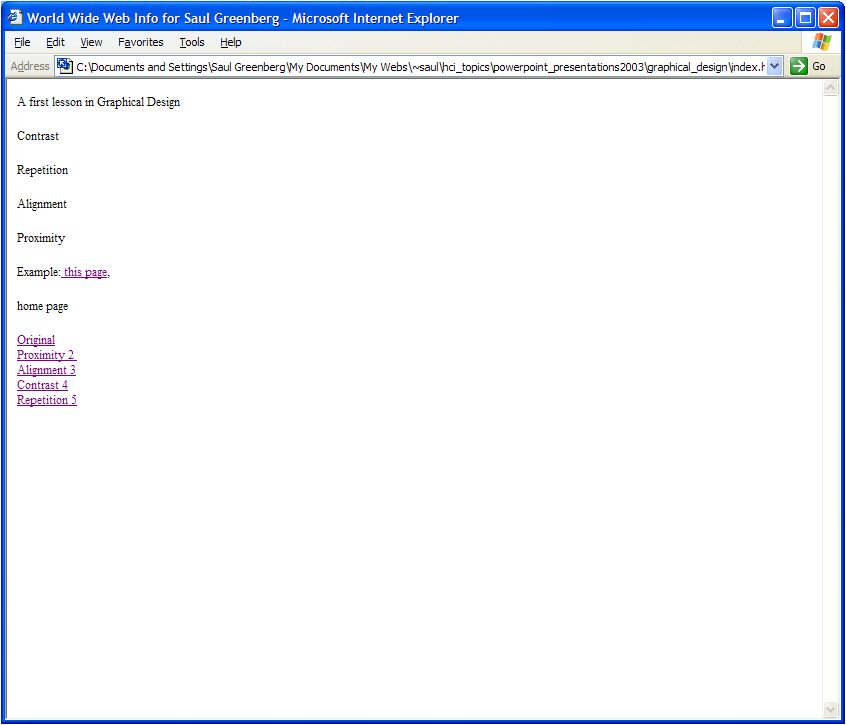
\includegraphics[scale=0.5]{1.png}}}
    \end{picture}
    
    \begin{tikzpicture}
	\put(230,-140){\node[draw][scale=1.7, fill=white] at (0,0) {\textbf{Original}};}
	\end{tikzpicture}    
    
\end{frame}



{\setbeamercolor{background canvas}{bg=fundal}
\begin{frame}
	
     \begin{picture}(0,0)
        \put(17,-168){\hbox{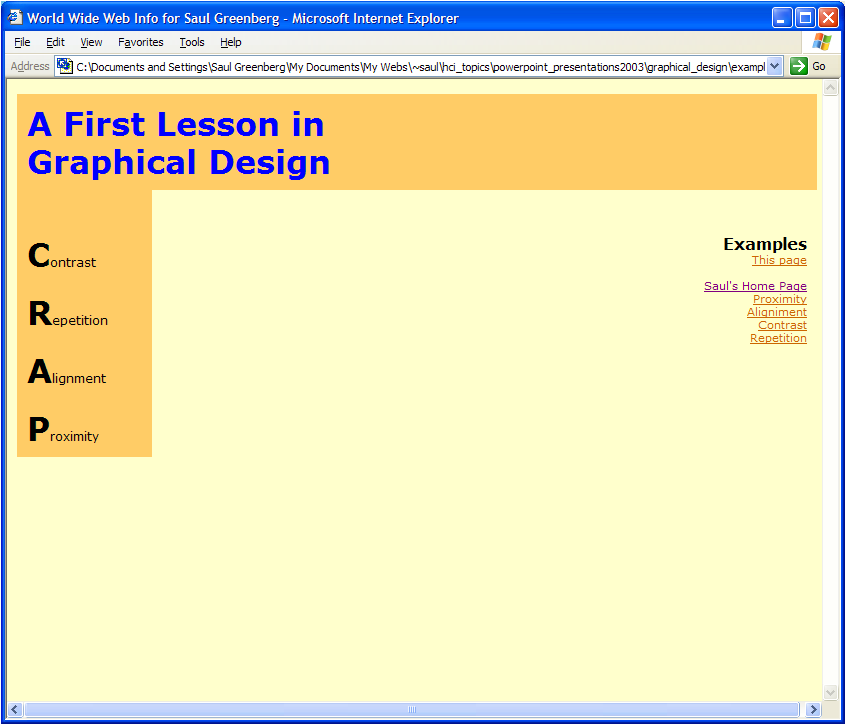
\includegraphics[scale=0.5]{2.png}}}
    \end{picture}

    \begin{tikzpicture}
	\put(230,-140){\node[draw][scale=1.7, fill=white] at (0,0) {\textbf{CRAP}};}
	\end{tikzpicture}

\end{frame}



{\setbeamercolor{background canvas}{bg=fundal}
\begin{frame}
	
     \begin{picture}(0,0)
        \put(17,-168){\hbox{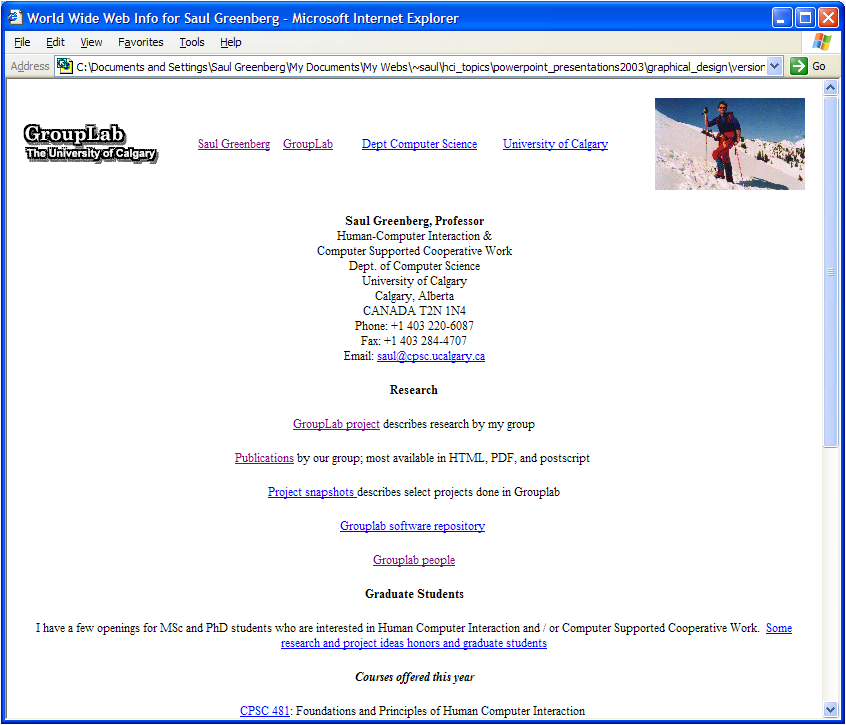
\includegraphics[scale=0.5]{3.png}}}
    \end{picture}
    
    \begin{tikzpicture}
	\put(230,-140){\node[draw][scale=1.7, fill=white] at (0,0) {\textbf{Original}};}
	\end{tikzpicture}

\end{frame}



{\setbeamercolor{background canvas}{bg=fundal}
\begin{frame}
	
     \begin{picture}(0,0)
        \put(17,-168){\hbox{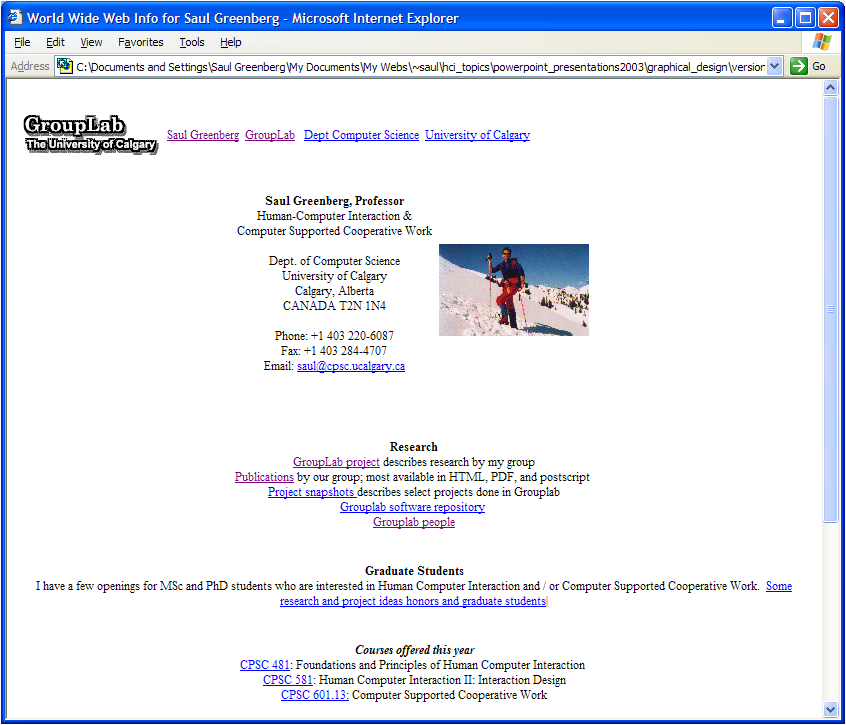
\includegraphics[scale=0.5]{4.png}}}
    \end{picture}
    
    \begin{tikzpicture}
	\put(230,-140){\node[draw][scale=1.7, fill=white] at (0,0) {\textbf{Proximity}};}
	\end{tikzpicture}

\end{frame}



{\setbeamercolor{background canvas}{bg=fundal}
\begin{frame}
	
     \begin{picture}(0,0)
        \put(17,-168){\hbox{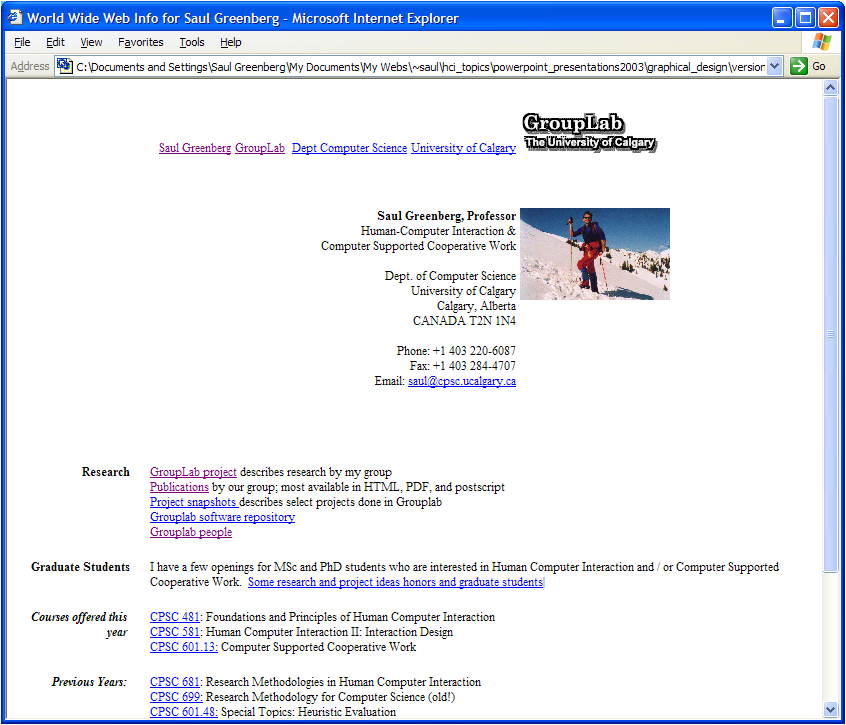
\includegraphics[scale=0.5]{5.png}}}
    \end{picture}
    
    \begin{tikzpicture}
	\put(230,-140){\node[draw][scale=1.7, fill=white] at (0,0) {\textbf{Alignment}};}
	\end{tikzpicture}

\end{frame}



%Hrab Constantin-Cristian
%8
{\setbeamercolor{background canvas}{bg=fundal}
\begin{frame}
	
     \begin{picture}(0,0)
        \put(17,-168){\hbox{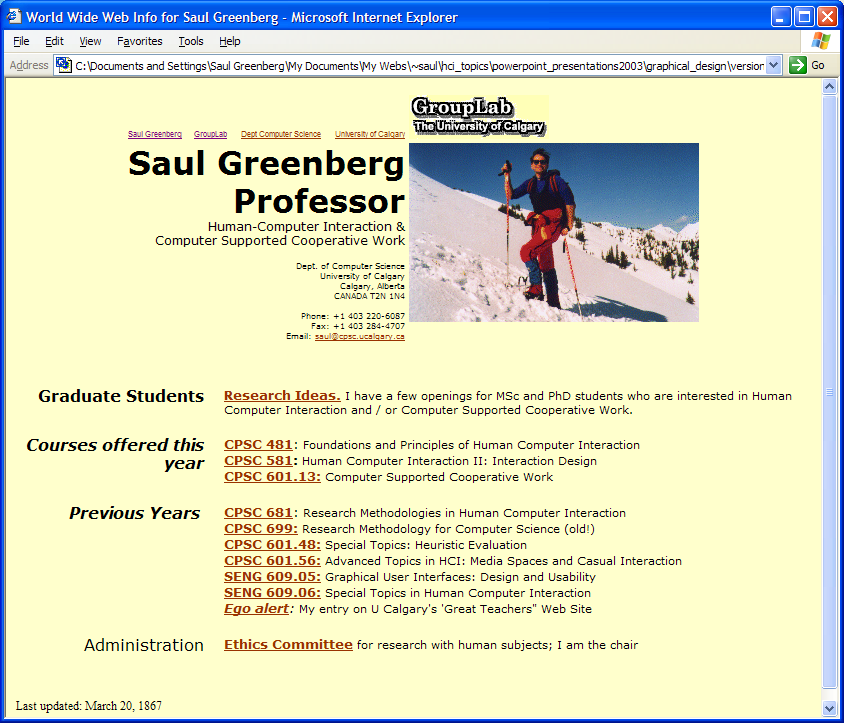
\includegraphics[scale=0.5]{8_picture1.png}}}
    \end{picture}
    
    \begin{tikzpicture}
	\put(230,-140){\node[draw][scale=1.7, fill=white] at (0,0) {\textbf{Contrast}};}
	\end{tikzpicture}

\end{frame}



%Hrab Constantin-Cristian
%9
{\setbeamercolor{background canvas}{bg=fundal}
\begin{frame}
	
     \begin{picture}(0,0)
        \put(17,-169.5){\hbox{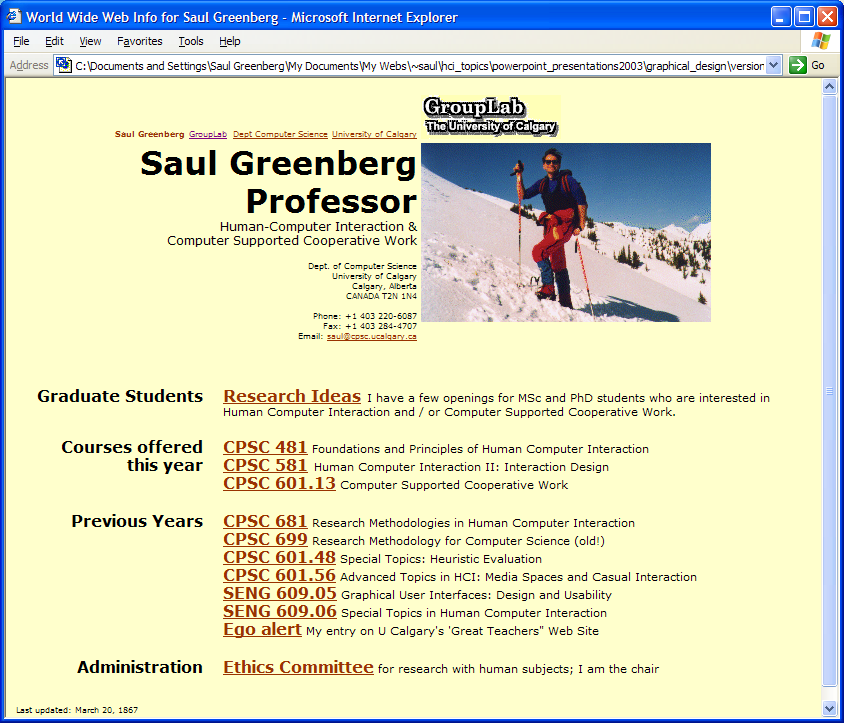
\includegraphics[scale=0.5]{9_picture2.png}}}
    \end{picture}
    
    \begin{tikzpicture}
	\put(230,-140){\node[draw][scale=1.7, fill=white] at (0,0) {\textbf{Repetition}};}
	\end{tikzpicture}

\end{frame}



%Hrab Constantin-Cristian
%10
{\setbeamercolor{background canvas}{bg=fundal}
\begin{frame}
{\textbf{Grids}}{\textcolor{red}{\rule{12cm}{1.2pt}}}

	{Horizontal and vertical lines to locate window components}
	 \begin{itemize}
      \item[--]{aligns related components} \newline
    \end{itemize} 
    {Organization}
    \setlist{nosep}
     \begin{enumerate}
      \item[--]{contrast for dominant elements}
      \item[--]{element groupings by proximity} 
      \item[--]{organizational structure}
      \item[--]{alignment} \newline
    \end{enumerate} 
    {Consistency}
    \setlist{nosep}
	 \begin{enumerate}
      \item[--]{location} 
      \item[--]{format} 
      \item[--]{element repetition} 
      \item[--]{organization} 
    \end{enumerate} 
    
     \begin{tikzpicture}
     \put(170,150){
     \draw [black](0,0) rectangle (4.7,3.7); \draw[gray] (0.2,0.2) rectangle (4.5,3.5);
      \draw[gray, ultra thin] (0.2,0.8) -- (4.5,0.8);  \draw[gray, ultra thin] (0.2,0.9) -- (4.5,0.9);
       \draw[gray, ultra thin] (0.2,2.5) -- (4.5,2.5);  \draw[gray, ultra thin] (0.2,2.6) -- (4.5,2.6);
       
        \draw[gray, ultra thin] (0.8,0.2) -- (0.8,3.5); \draw[gray, ultra thin] (0.9,0.2) -- (0.9,3.5);
        \draw[gray, ultra thin] (1.5,0.2) -- (1.5,3.5); \draw[gray, ultra thin] (1.6,0.2) -- (1.6,3.5);
          \draw[gray, ultra thin] (2.2,0.2) -- (2.2,3.5); \draw[gray, ultra thin] (2.3,0.2) -- (2.3,3.5);
            \draw[gray, ultra thin] (2.9,0.2) -- (2.9,3.5); \draw[gray, ultra thin] (3,0.2) -- (3,3.5);
           \draw[gray, ultra thin] (3.7,0.2) -- (3.7,3.5); \draw[gray, ultra thin] (3.8,0.2) -- (3.8,3.5);
     
     	\draw[black, thick] (0.2,2.6) rectangle (1.5,3.5);
        \draw[black, thick] (1.6,0.9) rectangle (4.5,3.5);
         \draw[black, thick] (1.6,0.2) rectangle (2.9,0.8);
         \draw[black, thick] (3,0.2) rectangle (4.5,0.8);
         
          \draw[gray, dashed, ultra thin ] (3.1,0.3) rectangle (4.4,0.7);
          
          \node[scale=0.7, black] at (0.8,3.2) {\textbf{Standard}};
          \node[scale=0.7, black] at (0.8,2.9) {\textbf{icon set}};
          
           \node[scale=0.7, black] at (2.6,3.3) {Message text in};
            \node[scale=0.7, black] at (2.4,3) {Arial 14, left };
            \node[scale=0.7, black] at (2.2,2.7) {adjusted };
            
            \node[scale=0.8, black] at (2.2,0.5) {\textbf{No}};
            \node[scale=0.8, black] at (3.7,0.5) {\textbf{Ok}};
            \draw[red] (1.3,3.2) -- (2.52,4.68);
            \draw[red] (3.2,0.5) -- (2.55,-0.4);

            }
	\end{tikzpicture}
   	\vspace{-218px}
    {
    
    \hspace{119px}{\vspace{5px}\textbox{Widget to widget spacing}{5em}{0.7}{1.1}{-0.9}}
   
    
    }
    \vspace{10px}
    {
    
    \hspace{98px}{\vspace{5px}\textbox{Window to widget spacing}{5em}{0.7}{1.1}{0.5}}
    
    }
	\vspace{-183px}
    {
    
    \hspace{230px}{\vspace{5px}\textboxSTG{Format of variable contents}{5em}{-0.7}{-1.1}{-1.5}}
    
    }
    
	\vspace{80px}
    {
    
    \hspace{233px}{\vspace{5px}\textboxSTG{Fixed components}{5em}{-0.7}{-1}{0.55}}
    
    }
  
  	\vspace{170px}

     \AddToShipoutPictureFG*{
    \AtPageLowerLeft{\put(-2,2){\makebox[\paperwidth][r]{\fontsize{4pt}{1pt}\selectfont{\color{gray}{Saul Greenberg}}}}}  
    }
\end{frame}



%Hrab Constantin-Cristian
%11
{\setbeamercolor{background canvas}{bg=fundal}
\begin{frame}
 \begin{tikzpicture}
     \put(0,30){
     \draw [black](0,0) rectangle (4.7,3.7); \draw[gray] (0.2,0.2) rectangle (4.5,3.5);
      \draw[gray, ultra thin] (0.2,0.8) -- (4.5,0.8);  \draw[gray, ultra thin] (0.2,0.9) -- (4.5,0.9);
       \draw[gray, ultra thin] (0.2,2.5) -- (4.5,2.5);  \draw[gray, ultra thin] (0.2,2.6) -- (4.5,2.6);
       
        \draw[gray, ultra thin] (0.8,0.2) -- (0.8,3.5); \draw[gray, ultra thin] (0.9,0.2) -- (0.9,3.5);
        \draw[gray, ultra thin] (1.5,0.2) -- (1.5,3.5); \draw[gray, ultra thin] (1.6,0.2) -- (1.6,3.5);
          \draw[gray, ultra thin] (2.2,0.2) -- (2.2,3.5); \draw[gray, ultra thin] (2.3,0.2) -- (2.3,3.5);
            \draw[gray, ultra thin] (2.9,0.2) -- (2.9,3.5); \draw[gray, ultra thin] (3,0.2) -- (3,3.5);
           \draw[gray, ultra thin] (3.7,0.2) -- (3.7,3.5); \draw[gray, ultra thin] (3.8,0.2) -- (3.8,3.5);
     
     	\draw[black, thick] (0.2,2.6) rectangle (1.5,3.5);
        \draw[black, thick] (1.6,0.9) rectangle (4.5,3.5);
         \draw[black, thick] (1.6,0.2) rectangle (2.9,0.8);
         \draw[black, thick] (3,0.2) rectangle (4.5,0.8);
         
          \draw[gray, dashed, ultra thin ] (3.1,0.3) rectangle (4.4,0.7);
          
          \node[scale=0.7, black] at (0.8,3.2) {\textbf{Standard}};
          \node[scale=0.7, black] at (0.8,2.9) {\textbf{icon set}};
          
           \node[scale=0.7, black] at (2.6,3.3) {Message text in};
            \node[scale=0.7, black] at (2.4,3) {Arial 14, left };
            \node[scale=0.7, black] at (2.2,2.7) {adjusted };
            
            \node[scale=0.8, black] at (2.2,0.5) {\textbf{No}};
            \node[scale=0.8, black] at (3.7,0.5) {\textbf{Ok}};
            
            \draw [cyan, -latex, ultra thick] (4.8,1.5) -- (6.3,1.5);
            \draw [cyan, -latex, ultra thick] (4.8,1.5) -- (6.3,-2.5);
            }
            
            \put(180,30){
     \draw [black](0,0) rectangle (4.7,3.7); 
     
     
     	\draw[black, thick] (0.2,2.6) rectangle (1.5,3.5);
        \draw[black, thick] (1.6,0.9) rectangle (4.5,3.5);
         \draw[black, thick] (1.6,0.2) rectangle (2.9,0.8);
         \draw[black, thick] (3,0.2) rectangle (4.5,0.8);
         
          \draw[gray, dashed, ultra thin ] (3.1,0.3) rectangle (4.4,0.7);
          
          \node[scale=2.2, black] at (0.8,3) {\textbf{?}}; 
          
           \node[scale=0.85, black] at (2.95,3.3) {Do you really want};
           \node[scale=0.85, black] at (2.8,2.9) {to delete the file};
           \node[scale=0.85, black] at (2.85,2.5) {“myfile.doc” from};
           \node[scale=0.85, black] at (2.85,2.1) {the folder “junk”?};
            
            \node[scale=0.8, black] at (2.2,0.5) {\textbf{No}};
            \node[scale=0.8, black] at (3.7,0.5) {\textbf{Ok}};
            }
            \put(180,-90){
     \draw [black](0,0) rectangle (4.7,3.7); 
     
     	\draw[black, thick] (0.2,2.6) rectangle (1.5,3.5);
        \draw[black, thick] (1.6,0.9) rectangle (4.5,3.5);
         \draw[black, thick] (3,0.2) rectangle (4.5,0.8);
         
          \draw[gray, dashed, ultra thin ] (3.1,0.3) rectangle (4.4,0.7);
          
          \node[scale=2.2, black] at (0.8,3) {\textbf{!}}; 
          
           \node[scale=0.85, black] at (2.85,3.3) {Cannot move the};
           \node[scale=0.85, black] at (2.9,2.9) {file “myfile.doc” to};
           \node[scale=0.85, black] at (2.8,2.5) {the folder “junk”};
           \node[scale=0.85, black] at (2.9,2.1) {because the disc is};
            \node[scale=0.85, black] at (1.9,1.7) {full.};
			\node[scale=0.8, black] at (3.7,0.5) {\textbf{Ok}};
            \node[scale=0.8, black] at (2.5,-0.5) {\CheckmarkBold};
            }
            
  \put(0,-90){
     \draw [black](0,0) rectangle (4.7,3.2); 
     	
        \draw[black, thick] (0.2,0.9) rectangle (3,2);
         \draw[black, thick] (3.1,0.6) rectangle (4.5,1.2);
         \draw[black, thick] (3.1,1.6) rectangle (4.5,2.2);
         
           \node[scale=0.85, black] at (1.05,1.7) {The file was};
           \node[scale=0.85, black] at (0.9,1.4) {destroyed};

			\node[scale=0.8, black] at (3.8,0.9) {\textit{\textbf{Cancel}}};
            \node[scale=0.8, black] at (3.8,1.9) {Apply};
            \node[scale=0.8, black] at (2.5,-0.5) {\ding{55}};
            }
            
      \begin{picture}(0,0)
        \put(10,-30){\hbox{
\includegraphics[scale=0.45]{11_picture.png}}}
    \end{picture}
    
	\end{tikzpicture}
\end{frame}



%Hrab Constantin-Cristian
%12
\newcommand\sbullet[1][.5]{\mathbin{\vcenter{\hbox{\scalebox{#1}{$\bullet$}}}}}
{\setbeamercolor{background canvas}{bg=fundal}
\begin{frame}

\begin{tikzpicture}
	\begin{picture}(0,0)
        \put(155,-130){\hbox{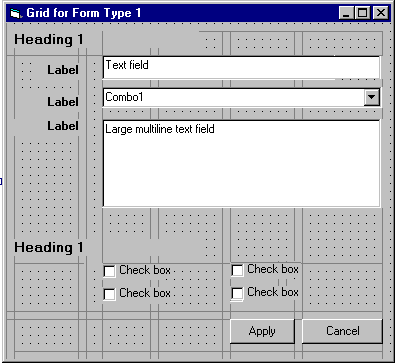
\includegraphics[scale=0.5]{12_picture1.png}} 
        }
    \end{picture}
    
    \begin{picture}(0,0)
        \put(355,-130){\hbox{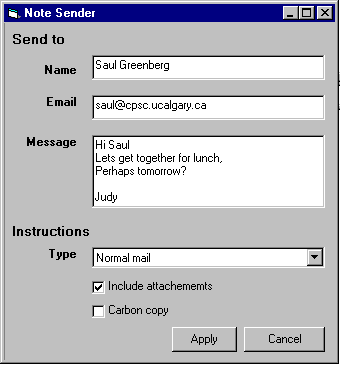
\includegraphics[scale=0.5]{12_picture2.png}}}
    \end{picture}
    	
\put(145,-100){ \draw [red, -latex, ultra thick] (5.8,1.5) -- (7,1.5);	
     
    }
\end{tikzpicture}

    \vspace{-10px}
    {
    \hspace{0px}{ \vspace{5px} \textboxSTG{Two-level Hierarchy $\newline \bullet$indentation$\linebreak \bullet$contrast}{10em}{-1.5}{-2}{-2}}

    }
    \vspace{-60px}
    {
    \hspace{180px}{ \vspace{5px} \textboxSTGA{Logic of organizational $\linebreak$flow}{10em}{-1}{-1}{-4}}    
    }
    
    \vspace{30px}
    {
    \hspace{18px}{ \vspace{5px} \textboxSTG{Alignment connects visual elements in a sequence }{10em}{-0.2}{-0.3}{+1.8}}  
    }

     \vspace{-140px}
    {
    \hspace{125px}{ \vspace{5px} \textboxSTG{Grouping by white space}{7em}{-0.2}{-0.2}{+3.8}}
	}
        
\end{frame}



%Hrab Constantin-Cristian
%13
{\setbeamercolor{background canvas}{bg=fundal}
\begin{frame}
{\textbf{Visual consistency (repetition)}}{\textcolor{red}{\rule{12cm}{1.2pt}}}

\vspace{-1.5cm}

	{internal consistency}
	 \begin{itemize}
      \item[--]{elements follow same conventions and rules}
      \item[--]{set of application-specific grids enforce this} 
      \newline
    \end{itemize} 
    
    {external consistency}
    \setlist{nosep}
     \begin{enumerate}
      \item[--]{follow platform and interface style conventions}
      \item[--]{use platform and widget-specific grids}
      \newline
    \end{enumerate} 
    
    {deviate only when it provides a clear benefit to user }

\vspace{-0.7cm}
    
    \begin{tikzpicture}
   		\begin{picture}(0,0)
        	\put(0,-100){\hbox{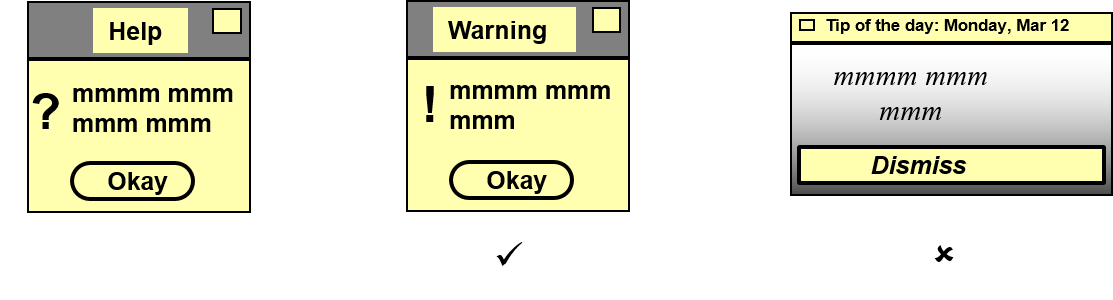
\includegraphics[scale=0.55]{13_picture.png}} 
        	}
    	\end{picture}
    
      \end{tikzpicture}
     \AddToShipoutPictureFG*{
    \AtPageLowerLeft{\put(-2,2){\makebox[\paperwidth][r]{\fontsize{4pt}{1pt}\selectfont{\color{gray}{Saul Greenberg}}}}}  
    }
\end{frame}



%Hrab Constantin-Cristian
%14
{\setbeamercolor{background canvas}{bg=fundal}
\begin{frame}
{\textbf{Relating screen elements}}{\textcolor{red}{\rule{12cm}{1.2pt}}}

\vspace{-2.5cm}

	{proximal clusters} \newline
    {alignment} \newline
    {white (negative) space}\newline
    {explicit structure}\newline
	
    \begin{tikzpicture}
   		\begin{picture}(0,0)
        	\put(0,-120){\hbox{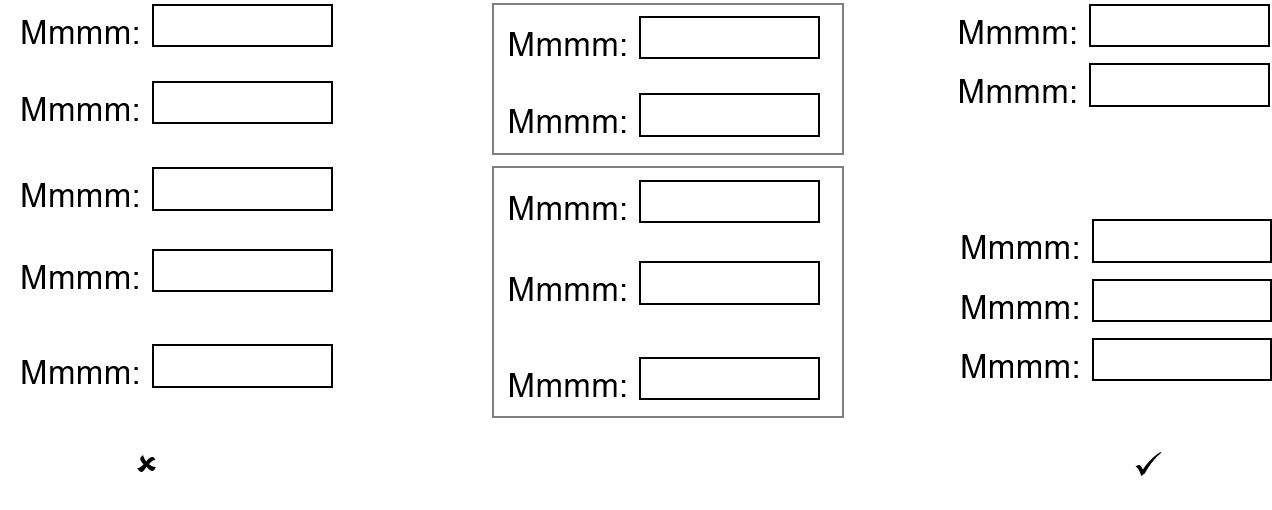
\includegraphics[scale=0.5]{14_picture.png}} 
        	}
    	\end{picture}
    
      \end{tikzpicture}
     \AddToShipoutPictureFG*{
    \AtPageLowerLeft{\put(-2,2){\makebox[\paperwidth][r]{\fontsize{4pt}{1pt}\selectfont{\color{gray}{Saul Greenberg}}}}}  
    }
\end{frame}



%Lotan Andrei
%Numarul slide-ului:23
\begin{frame}
{\textbf{Navigational cues}}{\textcolor{red}{\rule{12cm}{1.2pt}}}

    {provide initial focus} \newline \newline
	direct attention as appropriate to important, secondary, or \newline 
    peripheral items as appropriate \newline \newline
order should follow a user’s conceptual model of sequences \newline \newline

    \vspace{50px}
    \begin{picture}(0,0)
        \put(15,-30){\hbox{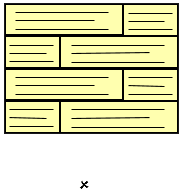
\includegraphics[scale=0.67]{23_picture1.png}}}
    \end{picture}
     \begin{picture}(0,0)
        \put(145,-28){\hbox{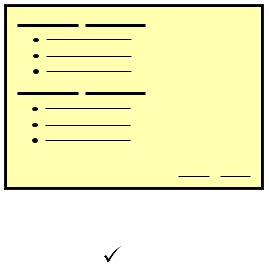
\includegraphics[scale=0.47]{23_picture2.png}}}
    \end{picture}
    
    \vspace{30px}
   \AddToShipoutPictureFG*{
    	\AtPageLowerLeft{\put(-2,2){\makebox[\paperwidth][r]{\fontsize{4pt}{1pt}\selectfont{\color{gray}{Saul Greenberg}}}}}  
    }
\end{frame}



%Lotan Andrei
%Numarul slide-ului:26
\begin{frame}
{\textbf{Economy of visual elements}}{\textcolor{red}{\rule{12cm}{1.2pt}}}

    {minimize number of controls} 
    \newline

	{include only those that are necessary}
	 \begin{itemize}
      \item[--]{eliminate, or relegate others to secondary windows} 	  \newline
    \end{itemize} 

    {minimize clutter}
     \begin{itemize}
      \item[--]{so information is not hidden} 
      \newline
    \end{itemize} 

    \vspace{60px}
    
    \begin{picture}(0,0)
        \put(45,-40){\hbox{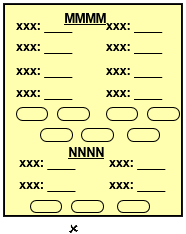
\includegraphics[scale=0.67]{26_picture1.png}}}
    \end{picture}
     \begin{picture}(0,0)
        \put(175,-40){\hbox{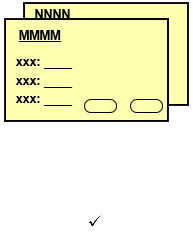
\includegraphics[scale=0.67]{26_picture2.png}}}
    \end{picture}
    
    \vspace{40px}
    \AddToShipoutPictureFG*{
    	\AtPageLowerLeft{\put(-2,2){\makebox[\paperwidth][r]{\fontsize{4pt}{1pt}\selectfont{\color{gray}{Saul Greenberg}}}}}  
    }
\end{frame}



%Neacsu Madalin
%Numarul slide-ului:29
\begin{frame}
{\textbf{Legibility and readability}}{\textcolor{red}{\rule{12cm}{1.2pt}}}

\Large{Characters, symbols, graphical elements should be easily noticable and distinguishable }

\vspace{16pt}

\begin{tabular}{cc}
\begin{minipage}{140pt}

\centering

\hvtext{\LARGE{Text set in\\
 Helvetica}} \\

\vspace{10pt}

\timestext{\LARGE{Text set in\\
 Times Roman}} \\
\vspace{15pt}
\checkmark
\end{minipage} &

\begin{minipage}{140pt}

\centering
\LARGE{TEXT SET IN \\
CAPITALS}\\

\vspace{7pt}

\LARGE\rtndfamily{{Text set in \\
Braggadocio}}\\
\vspace{7pt}

\LARGE{\texttt{Text set in \\
Courier}}\\

\vspace{7pt}

\ding{56}
\end{minipage}
\end{tabular}

\begin{textblock*}{60pt}(315pt, 260pt)
\tiny{\transpt{Saul Greenberg}}
\end{textblock*}

\end{frame}



%Neacsu Madalin
%Numarul slide-ului:30
\begin{frame}
{\textbf{Legibility and readability}}{\textcolor{red}{\rule{12cm}{1.2pt}}}

Proper use of typography
\begin{itemize}
\item[--] 1 - 2 typefaces (3 max)
\item[--] normal, italics, bold
\item[--] 1 - 3 sizes max

\end{itemize}

\vspace{6pt}


\begin{tabular}{cc}
\begin{minipage}{140pt}
\textbf{\LARGE{Large}\\
 \large{Medium}\\
 \small{Small}
}

\end{minipage} &

\begin{minipage}{140pt}
\textbf{\Large{Large}\\
 \large{Medium}\\
 \normalsize{Small}
}
\end{minipage}

\end{tabular}
\vspace{4pt}

\begin{tabular}{cc}
\begin{minipage}{140pt}
\raggedright{\large{\textbf{ Readable}}} \\
\vspace{4pt}
\centering
\textbf{Design components to be \\
 inviting and attractive \\
\
Design components to be \\
 inviting and attractive \\
}

\vspace{4pt}

\checkmark

\end{minipage} &
\begin{minipage}{140pt}
\textbf{\underline{\Large{\it Unreadable}}}\\
  Design components to be \\
  {\it inviting} and \underline{attractive} \\

 \large{Design components to be\\
 \textcolor{red}{inviting} and \textcolor{red}{\it attractive}}\\

\vspace{4pt}

\centering
\ding{56}
\end{minipage}

\end{tabular}

\begin{textblock*}{60pt}(315pt, 260pt)
\tiny{\transpt{Saul Greenberg}}
\end{textblock*}

\end{frame}



%Neacsu Madalin
%Numarul slide-ului:31
\begin{frame}
{\textbf{Legibility and readability}}{\textcolor{red}{\rule{12cm}{1.2pt}}}

typesetting
\begin{itemize}
\item[--] point size
\item[--] word and line spacing
\item[--] line length
\item[--] indentation
\item[--] color

\end{itemize}

\vspace{6pt}

\begin{tabular}{cc}
\begin{minipage}{140pt}
\raggedright{\textbf{ Readable:}} \\
\vspace{4pt}
\centering
\textbf{Design components to be \\
 inviting and attractive \\
\
Design components to be \\
 inviting and attractive \\
}

\vspace{4pt}

\checkmark

\end{minipage} &

\begin{minipage}{160pt}
\transpt{Unreadable:  Design components \\
to be  easy to interpret and \\
understand. Design components to \\
be inviting and attractive\\

\vspace{4pt}
}
\centering
\ding{56}
\end{minipage}

\end{tabular}

\begin{textblock*}{60pt}(315pt, 260pt)
\tiny{\transpt{Saul Greenberg}}
\end{textblock*}
\end{frame}



%Ionel Andrei-Stefan
%Numarul slide-ului:15
{\setbeamercolor{background canvas}{bg=fundal}
\begin{frame}
{\textbf{Example}}{\textcolor{red}{\rule{12cm}{1.2pt}}}

	\begin{figure}
        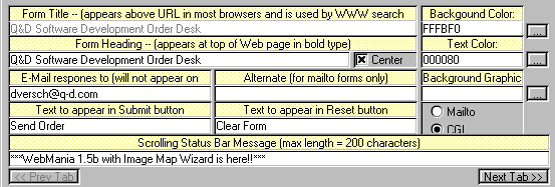
\includegraphics[scale=0.45]{15_picture.png}
    \end{figure}

\vspace{80px}\hspace{-25px}\fontsize{8pt}{1pt}\selectfont{\color{gray}{Webforms}} 
\end{frame}



{\setbeamercolor{background canvas}{bg=fundal}
\begin{frame}
{\textbf{Example}}{\textcolor{red}{\rule{12cm}{1.2pt}}}

    {Terrible alignment}
	\begin{itemize}
      	\item[--]\small{no flow}
      	\newline
    \end{itemize} 
    
    {Poor contrast}
	\begin{itemize}
      	\item[--]\small{cannot distinguish colored labels from editable fields}
      	\newline
    \end{itemize} 
    
    {Poor repetition}
	\begin{itemize}
      	\item[--]\small{buttons do not look like buttons}
      	\newline
    \end{itemize} 
    
    {Poor explicit structure}
	\begin{itemize}
      	\item[--]\small{blocks compete with alignment}
      	\newline
    \end{itemize} 
    
    \vspace{20px}

    \AddToShipoutPictureFG*{
    	\AtPageLowerLeft{\put(-2,2){\makebox[\paperwidth][r]{\fontsize{4pt}{1pt}\selectfont{\color{gray}{Saul Greenberg}}}}}  
    }
\end{frame}



%Ionel Andrei-Stefan
%Numarul slide-ului:16
{\setbeamercolor{background canvas}{bg=fundal}
\begin{frame}
{\textbf{Example}}{\textcolor{red}{\rule{12cm}{1.2pt}}}

\begin{figure}
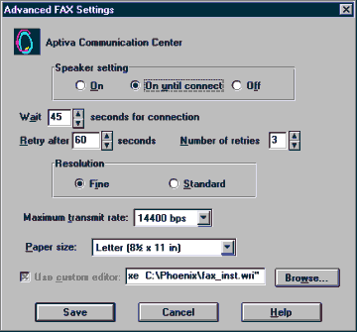
\includegraphics[scale=0.4]{16_picture.png}
\end{figure}

{No regard for order and organization}

\vspace{5px}\hspace{-25px}\fontsize{8pt}{1pt}\selectfont{\color{gray}{IBM's Aptiva Communication Center}} 

\end{frame}



%Lotan Andrei
%Numarul slide-ului:28
\begin{frame}
{\textbf{Example}}{\textcolor{red}{\rule{12cm}{1.2pt}}}
    
    \begin{picture}(0,0)
        \put(10,-140){\hbox{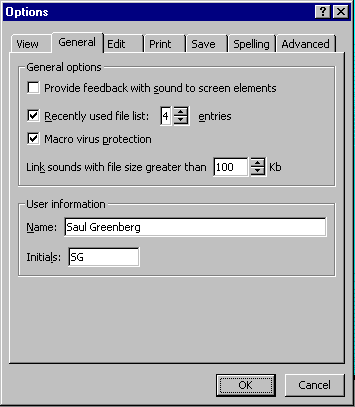
\includegraphics[scale=0.5]{28_picture1.png}}}
    \end{picture}
     \begin{picture}(0,0)
        \put(160,-140){\hbox{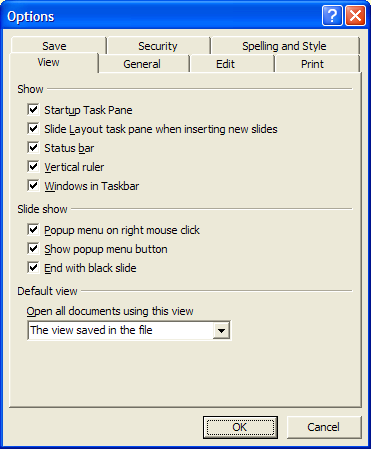
\includegraphics[scale=0.45]{28_picture2.png}}}
    \end{picture}
    
    \vspace{140px}
    \textbf{Tabs}
     \begin{itemize}
      \item[--]{excellent means for factoring related items}
      \item[--]{but can be overdone}
    \end{itemize} 
    
    \AddToShipoutPictureFG*{
    	\AtPageLowerLeft{\put(-2,2){\makebox[\paperwidth][r]{\fontsize{4pt}{1pt}\selectfont{\color{gray}{Saul Greenberg}}}}}  
    }

\end{frame}



%Neacsu Madalin
%Numarul slide-ului:33
\begin{frame}
{\textbf{Example}}{\textcolor{red}{\rule{12cm}{1.2pt}}}

\vspace{-1.5cm}

\centering
\begin{overpic}[width=11cm, height=4cm]{33_Time_Chaos_wg}
\put(85, -16){\line(1, 0){5}}
\put(90, -16){\vector(0, 1 ){31}}
\put(-6, -16){\minibox[frame]{\Large{\textbf{These choices must be really important,}}\\ \Large{\textbf{or are they?}}}}
\end{overpic}
\end{frame}



%Neacsu Madalin
%Numarul slide-ului:34
\begin{frame}
{\textbf{Example}}{\textcolor{red}{\rule{12cm}{1.2pt}}}

\vspace{2cm}

\centering
\begin{overpic}[width=10cm, height=3.5cm]{34_RpW95}

\put(8, 48){\line(1, 0){4}}
\put(8, 48){\vector(1, -2 ){11.3}}

\put(12, 48){\minibox[frame]{\Large{\textbf{Greyed-out example text hard to read.}}\\ \Large{\textbf{Why not make it black?}}}}
\end{overpic}
\end{frame}



%Neacsu Madalin
%Numarul slide-ului:35
\begin{frame}
{\textbf{Example}}{\textcolor{red}{\rule{12cm}{1.2pt}}}

\centering
\begin{overpic}[width=2.2cm, height=7.5cm]{35_MsWord}
\put(-12, 26){\line(1, 0){7}}
\put(-5, 26){\vector(1, 2){13.7}}
\put(-67, 25){\minibox[frame]{\Large{\textbf{Text orientation}}\\ \Large{\textbf{difficult to read}}}}
\end{overpic}
\end{frame}



%Plesa Mihail
%Numarul slide-ului:36
\begin{frame}
{\textbf{Imagery}}{\textcolor{red}{\rule{12cm}{1.2pt}}}

	{Signs, icons, symbols}
	 \begin{itemize}
      \item[--]{right choice within spectrum from concrete to abstract} \newline
    \end{itemize} 
    {Icon design \textbf{very} hard}
     \begin{itemize}
      \item[--]{except for most familiar, always label them} \newline
    \end{itemize} 
    {Image position and type should be related}
	 \begin{itemize}
      \item[--]{image "family"} \newline
    \end{itemize} 
    {Consistent and relevant image use}
     \begin{itemize}
      \item[--]{identifies situations, offerings...} \newline
    \end{itemize}
    
    \begin{picture}(0,0)
        \put(275,30){\hbox{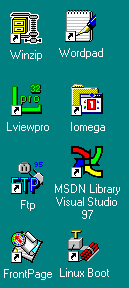
\includegraphics[scale=0.5]{36_picture1.png}}}
    \end{picture}
    
     \begin{picture}(0,0)
        \put(105,-35){\hbox{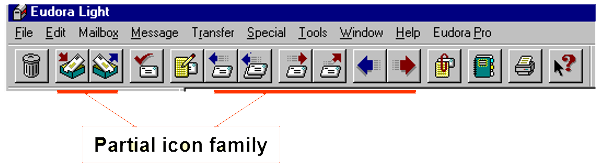
\includegraphics[scale=0.5]{36_picture2.png}}}
    \end{picture}
    
    \vspace{30px}
    \AddToShipoutPictureFG*{
    	\AtPageLowerLeft{\put(-2,2){\makebox[\paperwidth][r]{\fontsize{4pt}{1pt}\selectfont{\color{gray}{Saul Greenberg}}}}}
    }

\end{frame}



%Plesa Mihail
%Numarul slide-ului:39
\begin{frame}
{\textbf{Example}}{\textcolor{red}{\rule{12cm}{1.2pt}}}

\vspace{1cm}

    \begin{picture}(0,0)
        \put(20,-108){\hbox{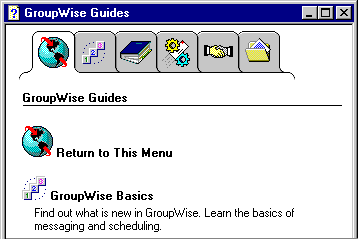
\includegraphics[scale=0.6]{39_picture.png}}}
    \end{picture}
    
    \vspace{105px}
    \hspace{23px}{What do these images mean? }
    \begin{itemize}
    	\addtolength{\itemindent}{10px}
      	\item[\textcolor{black}{•}]{no tooltips included}
      	\item[\textcolor{black}{•}]{one of the tabs is a glossary explaining these images! \\ \hspace{10px}Which one?}
    \end{itemize}
   
   \vspace{15px}
    \AddToShipoutPictureFG*{
    	\AtPageLowerLeft{\put(-2,2){\makebox[\paperwidth][r]{\fontsize{4pt}{1pt}\selectfont{\color{gray}{Saul Greenberg}}}}}
        \AtPageLowerLeft{\put(-285,5){\makebox[\paperwidth][r]{\fontsize{8pt}{1pt}\selectfont{\color{gray}{Novell GroupWise 5.1}}}}}  
    }
\end{frame}



%Plesa Mihail
%Numarul slide-ului:40
\begin{frame}
{\textbf{Idioms}}{\textcolor{red}{\rule{12cm}{1.2pt}}}

  	{Familiar ways of using GUI components}
     \begin{itemize}
      \item[--]{appropriate for casual to expert users}
      \item[--] {builds upon computer literacy}
      \item[--] {must be applied carefully in walk up and use systems}
    \end{itemize}
    \begin{picture}(0,0)
        \put(-15,-145){\hbox{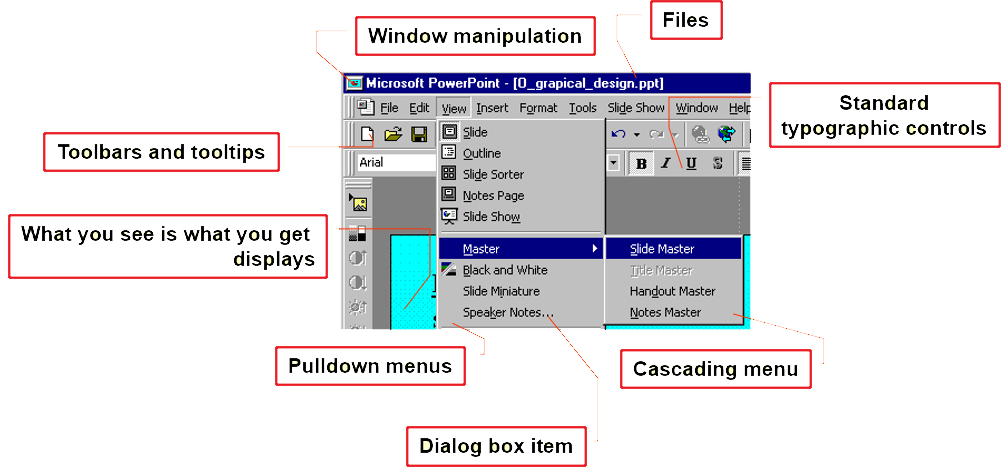
\includegraphics[scale=0.45]{40_picture.png}}}
    \end{picture}
    \vspace{125px}
    
    \AddToShipoutPictureFG*{
    	\AtPageLowerLeft{\put(-2,2){\makebox[\paperwidth][r]{\fontsize{4pt}{1pt}\selectfont{\color{gray}{Saul Greenberg}}}}}
        \AtPageLowerLeft{\put(-285,5){\makebox[\paperwidth][r]{\fontsize{8pt}{1pt}\selectfont{\color{gray}{Microsoft Powerpoint}}}}}  
    }

\end{frame}



%Plesa Mihail
%Numarul slide-ului:41
\begin{frame}
{\textbf{How to choose between widgets}}{\textcolor{red}{\rule{12cm}{1.2pt}}}

  	{What components must be in the display?}
    \begin{itemize}
    	\item[{--}]{ necessary visual affordances}
        \item[{--}]{ frequent actions}
        \begin{itemize}
        	\item[{•}]{direct manipulation for core activities}      
			\item[{•}]{buttons/forms/toolbar/special tools for frequent/immediate actions}
        	\item[{•}] {menus/property window for less frequent actions}
            \item[{•}] {secondary windows for rare actions}
        \end{itemize}
    \end{itemize}
    
    \vspace{20px}
    {How are components related?}
    \begin{itemize}
    	\item[{--}]{organize related items as "chunks"}
    \end{itemize}
    
     \vspace{20px}
    {What are familiar and expected idioms?}
    \begin{itemize}
    	\item[{--}]{cross application look and feel}
    \end{itemize}
    \vspace{40px}
	\AddToShipoutPictureFG*{
    	\AtPageLowerLeft{\put(-2,2){\makebox[\paperwidth][r]{\fontsize{4pt}{1pt}\selectfont{\color{gray}{Saul Greenberg}}}}}
    }
\end{frame}



%Raceanu Dragos
%Numarul slide-ului:43 
\begin{frame}
{\textbf{Widgets and complexity}}{\textcolor{red}{\rule{12cm}{1.2pt}}}

	\textbf{How can window navigation be reduced?}
	 \begin{itemize}
      \item[--]{avoid long paths}
       \item[--]{avoid deep hierarchies}
    \end{itemize} 
  \vspace{120px}

     \begin{picture}(0,0)
        \put(85,-30){\hbox{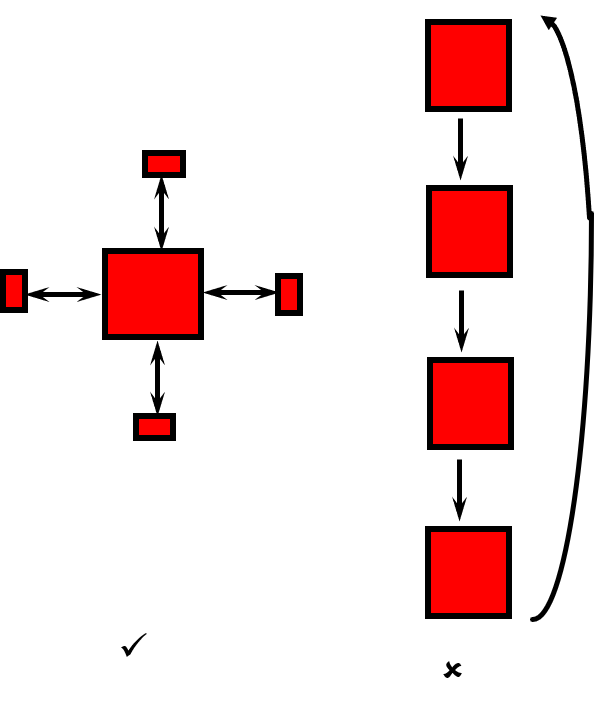
\includegraphics[scale=0.5]{43_picture.png}}}
    \end{picture}
    
    \vspace{25px}
     \AddToShipoutPictureFG*{
    	\AtPageLowerLeft{\put(-2,2){\makebox[\paperwidth][r]{\fontsize{4pt}{1pt}\selectfont{\color{gray}{Saul Greenberg}}}}}      
    }
\end{frame}



%Raceanu Dragos
%Numarul slide-ului:48
\begin{frame}
{\textbf{What you now know}}{\textcolor{red}{\rule{12cm}{1.2pt}}}

  	 \begin{itemize}
    	\item[] \textbf{{ CRAP}  }  
        \bigskip
        \item[] \textbf{{ Grids are an essential tool for graphical design} } 
        \bigskip
        \item[] \textbf{{ Other visual concepts include}}  
        \begin{itemize}
        \item[--] { visual consistency }
       		 \begin{itemize}
        	 \item[{•}]{ repetition}
             \end{itemize}
        \medskip
        \item[--] { visual organization }
       		 \begin{itemize}
        	 \item[{•}]{ contrast, alignment and navigational cues}
             \end{itemize}
              \medskip
        \item[--]{  visual relationships }
       		 \begin{itemize}
        	 \item[{•}]{ proximity and white space}
             \end{itemize}
              \medskip
        \item[--] { familiar idioms}
         \medskip
        \item[--] { legibility and readability}
       		 \begin{itemize}
        	 \item[{•}]{ typography}
             \end{itemize}
        \medskip      
        \item[--]{  appropriate imagery}


        \end{itemize}
    \end{itemize}
    \vspace{25px}
        \AddToShipoutPictureFG*{
    	\AtPageLowerLeft{\put(-2,2){\makebox[\paperwidth][r]{\fontsize{4pt}{1pt}\selectfont{\color{gray}{Saul Greenberg}}}}}
      
    }
  
\end{frame}



\usetikzlibrary{arrows,positioning} 
\tikzset{
    %Define style for boxes
    punkt/.style={
           rectangle,
           draw=blue, thick,
           minimum height=2em,
           text centered},
    dreptunghi/.style={
           rectangle,
           draw=black,
           minimum height=2em}
}

\newcommand{\sageatainsus}[7]{

\begin{tikzpicture}
        \node [single arrow,minimum width=#1, minimum height=#2,draw=black, rotate=#7,line width=#5,inner sep=#3] {   };
        \coordinate (P) at (0,0);
        \node[text width=#4] (N) at (P) {#6} ;
		
\end{tikzpicture}

}


%$ lungime text, grosime dreptunghi, text
\newcommand{\dreptunghi}[3]{

\begin{tikzpicture}
\node[dreptunghi,text width=#1,line width=#2] {#3};
\end{tikzpicture}

}
% culoare, grosime, lungime
\newcommand{\linie}[3]{
\begin{tikzpicture}
\draw[draw=#1,line width=#2] (0,0) -- (0,-#3) ;
\end{tikzpicture}
}


%spatiul intre linii
\renewcommand{\baselinestretch}{0.5} 

%Raceanu Dragos
%Numarul slide-ului:49
\begin{frame}
{\textbf{Interface Design and Usability Engineering}}{\textcolor{red}{\rule{12cm}{1.2pt}}}

\vspace{-48px}


 \begin{picture}(0,0)
        \put(26,-265){\hbox{
\includegraphics[scale=0.53]{49_picture.png}}}
 \end{picture}
 
  %%sagetile lipsa
\begin{picture}(0,0)
\put(118,-242){
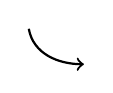
\begin{tikzpicture}
\draw [->,black,line width=0.8] (0,0) to [out=-80,in=180] (0.7,-0.45);
\end{tikzpicture}}
\put(118,-188){
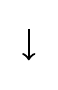
\begin{tikzpicture}
\draw [->,black,line width=0.8] (0,0) to (0,-0.4);
\end{tikzpicture}}

\put(212,-244){

\begin{tikzpicture}
\draw [->,black,line width=0.8] (0,0) to [out=-80,in=180] (0.5,-0.45);
\end{tikzpicture}}
\put(206,-188){
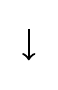
\begin{tikzpicture}
\draw [->,black,line width=0.8] (0,0) to (0,-0.4);
\end{tikzpicture}}
\end{picture}


% culoare, grosime, plecare (cu minus),lungime

\begin{picture}(0,0)
\put(90,-260){\linie{gray}{3}{8.5}}
\end{picture}


\begin{picture}(0,0)
\put(185,-247){\linie{gray}{3}{8.5}}
\end{picture}

\begin{picture}(0,0)
\put(270,-232){\linie{gray}{3}{8.5}}
\end{picture}

\vspace{-11px}


%%sus

\hspace{-29px}\textit{\textbf{\fontsize{9pt}{0pt}\selectfont{\color{black}Goals:
}}}

%dreaptunghiul 1
\begin{picture}(0,0)
\put(20,0)
{\dreptunghi{1.7cm}{0.6}{
\textbf{\fontsize{6pt}{0pt}\selectfont{\color{black}Articulate:\\
\textbullet who users are \\
\textbullet their key tasks
}}}}
\end{picture}



%dreptughiul 2
\begin{picture}(0,0)
\put(122,15)
{\dreptunghi{1.2cm}{0.6}{
\textbf{\fontsize{6pt}{0pt}\selectfont{\color{black}Brainstorm designs
}}}}
\end{picture}

%dreptughiul 3
\begin{picture}(0,0)
\put(212,30)
{\dreptunghi{1.2cm}{0.2}{
\textbf{\fontsize{6pt}{0pt}\selectfont{\color{black}Refined designs
}}}}
\end{picture}

%dreptughiul 4
\begin{picture}(0,0)
\put(285,42)
{\dreptunghi{1.1cm}{0.2}{
\textbf{\fontsize{6pt}{0pt}\selectfont{\color{gray}Completed designs
}}}}
\end{picture}


\vspace{30px}


%mij

\hspace{-29px}\textit{\textbf{\fontsize{8.5pt}{0pt}\selectfont{\color{black}Methods:
}}}

%sageata 1
\vspace{20px}
 \begin{picture}(0,0)
 \put(-4,-12){\sageatainsus{5.5em}{7.4em}{4mm}{1.25cm}{0.4}{\fontsize{6pt}{1pt}\selectfont{\color{black}Task centered system \vspace{4px} design 
Participatory  \vspace{4px} design
User-centered design}}{-90}}
 \end{picture}

%sageata 2
 \begin{picture}(0,0)
\put(47,7){\sageatainsus{1.8em}{6.8em}{4.5mm}{0.9cm}{0.6}{\fontsize{6pt}{0pt}\selectfont{\color{black} Evaluate tasks}}{90}}
 \end{picture}


%sageata 3
\begin{picture}(0,0)
\put(90,18){\sageatainsus{5em}{7em}{5mm}{1.3cm}{0.4}{
\textbf{\fontsize{6pt}{0pt}\selectfont{\color{black} Psychology of everyday \vspace{4px}  things}}

\fontsize{6pt}{0pt}\selectfont{\color{black} User \vspace{4px} involvement}

\textbf{\fontsize{6pt}{0pt}\selectfont{\color{black} Representation \& metaphors}}
}{-90}}
 \end{picture}
 
 
 %sageata 3 jos
\begin{picture}(0,0)
\put(90,-20){\sageatainsus{5em}{0em}{5mm}{1.2cm}{0.4}{
\textbf{\fontsize{6pt}{0pt}\selectfont{\color{black} low fidelity prototyping methods}}

}{-90}}
 \end{picture}
 
%sageata 4
\begin{picture}(0,0)
\put(137,50){\sageatainsus{4.5em}{7.4em}{5mm}{1.2cm}{0.4}{

\textit{\fontsize{6pt}{0pt}\selectfont{\color{black} Participatory \vspace{8px} interaction}}

\textit{\fontsize{6pt}{0pt}\selectfont{\color{black} Task scenario walk-through
}}

}{90}}
 \end{picture}

%sageata 5
\begin{picture}(0,0)
\put(185,60){\sageatainsus{4em}{7em}{5mm}{1cm}{0.4}{

\fontsize{6pt}{0pt}\selectfont{\color{red}Graphical screen  \vspace{4px} design}

\fontsize{6pt}{0pt}\selectfont{\color{gray}Interface \vspace{4px} guidelines}

\fontsize{6pt}{0pt}\selectfont{\color{gray}Style  \vspace{4px} guides}

}{-90}}
 \end{picture}
 
 
 %sageata 5 jos
\begin{picture}(0,0)
\put(185,20){\sageatainsus{5em}{4em}{5mm}{1.2cm}{0.4}{
\textbf{\fontsize{6pt}{0pt}\selectfont{\color{black} high fidelity prototyping methods}}

}{-90}}
 \end{picture}

%sageata 6
\begin{picture}(0,0)
\put(228,88){\sageatainsus{4em}{7em}{5mm}{1cm}{0.4}{

\textit{\fontsize{6pt}{0pt}\selectfont{\color{black} Usability
 \vspace{8px} testing}}

\textit{\fontsize{6pt}{0pt}\selectfont{\color{gray} Heuristic evaluation}}
}{90}}
 \end{picture}

%sageata 7
\begin{picture}(0,0)
\put(296,103){\sageatainsus{2.5em}{7em}{3.6mm}{0.7cm}{0.4}{

\textit{\fontsize{6pt}{0pt}\selectfont{\color{gray}Field testing}}
}{90}}
 \end{picture}
 
 
 
 \vspace{-39px}
 %%jos

\hspace{-29px}\vspace{25px}\textit{\textbf{\fontsize{9pt}{0pt}\selectfont{\color{black}Products:
}}}

%dreptunghiul 1
\begin{picture}(0,0)
\put(20,27)
{\dreptunghi{1.4cm}{0.2}{
\textbf{\fontsize{6pt}{0pt}\selectfont{\color{black}User and task descriptions
}}}}
\end{picture}

%dreptunghiul 2
\begin{picture}(0,0)
\put(120,40)
{\dreptunghi{1.4cm}{0.2}{
\textbf{\fontsize{6pt}{0pt}\selectfont{\color{black}Throw-away paper prototypes
}}}}
\end{picture}

%dreptunghiul 3
\begin{picture}(0,0)
\put(205,56)
{\dreptunghi{1.2cm}{0.2}{
\textbf{\fontsize{6pt}{0pt}\selectfont{\color{black}Testable prototypes
}}}}
\end{picture}

%dreptunghiul 4
\begin{picture}(0,0)
\put(280,60)
{\dreptunghi{1.4cm}{0.2}{
\textbf{\fontsize{6pt}{0pt}\selectfont{\color{gray}Alpha/beta systems or complete specification
}}}}
\end{picture}

\end{frame}



{\setbeamercolor{background canvas}{bg=background}
\begin{frame}
{\textbf{*Bibliography}}{\textcolor{red}{\rule{12cm}{1.2pt}}}

        \begin{itemize}
        	\item[{$\bullet$}] Saul Greenberg, \textbf{Designing and building visual interfaces. Graphical Screen Design}, University of Calgary, Canada

        	\url{http://pages.cpsc.ucalgary.ca/~saul/481/}
			\newline

			\item[{$\bullet$}] Keith Andrews, \textbf{Human Computer Interaction, Chapter 11. Visual Design and Typography, Chapter 12. Icon Design}, TU Graz, Austria

        	\url{https://courses.isds.tugraz.at/hci/hci.pdf}                			\newline
        	 
     	\end{itemize}
\end{frame}



{\setbeamercolor{background canvas}{bg=background}
\begin{frame}
{\textbf{*Bibliography}}{\textcolor{red}{\rule{12cm}{1.2pt}}}

        \begin{itemize}
        	\item[{$\bullet$}] Teo Siang, \textbf{Bad Design vs. Good Design: 5 Examples We can Learn From}
        	
        	\url{https://www.interaction-design.org/literature/article/bad-design-vs-good-design-5-examples-we-can-learn-frombad-design-vs-good-design-5-examples-we-can-learn-from-130706}
        	 \newline
        	 
        	 \item[{$\bullet$}] \textbf{6 Bad UI Design Examples \& Common Errors of UI Designers}
        	 
        	 \url{https://www.mockplus.com/blog/post/bad-ui-design-examples}
        	 \newline
        	 
        	 
     	\end{itemize}
\end{frame}



\end{document}